Lancer une partie pour jouer un morceau au piano, et gagnez le plus de points possible!
\\\\
Pour lancer une partie, sélectionnez d’abord une chanson depuis votre page personnelle (Voir Capture \ref{fig:access-song}), ou parmis les résultats d’une recherche (Voir Capture \ref{fig:search-song}).

\begin{figure}[H]
	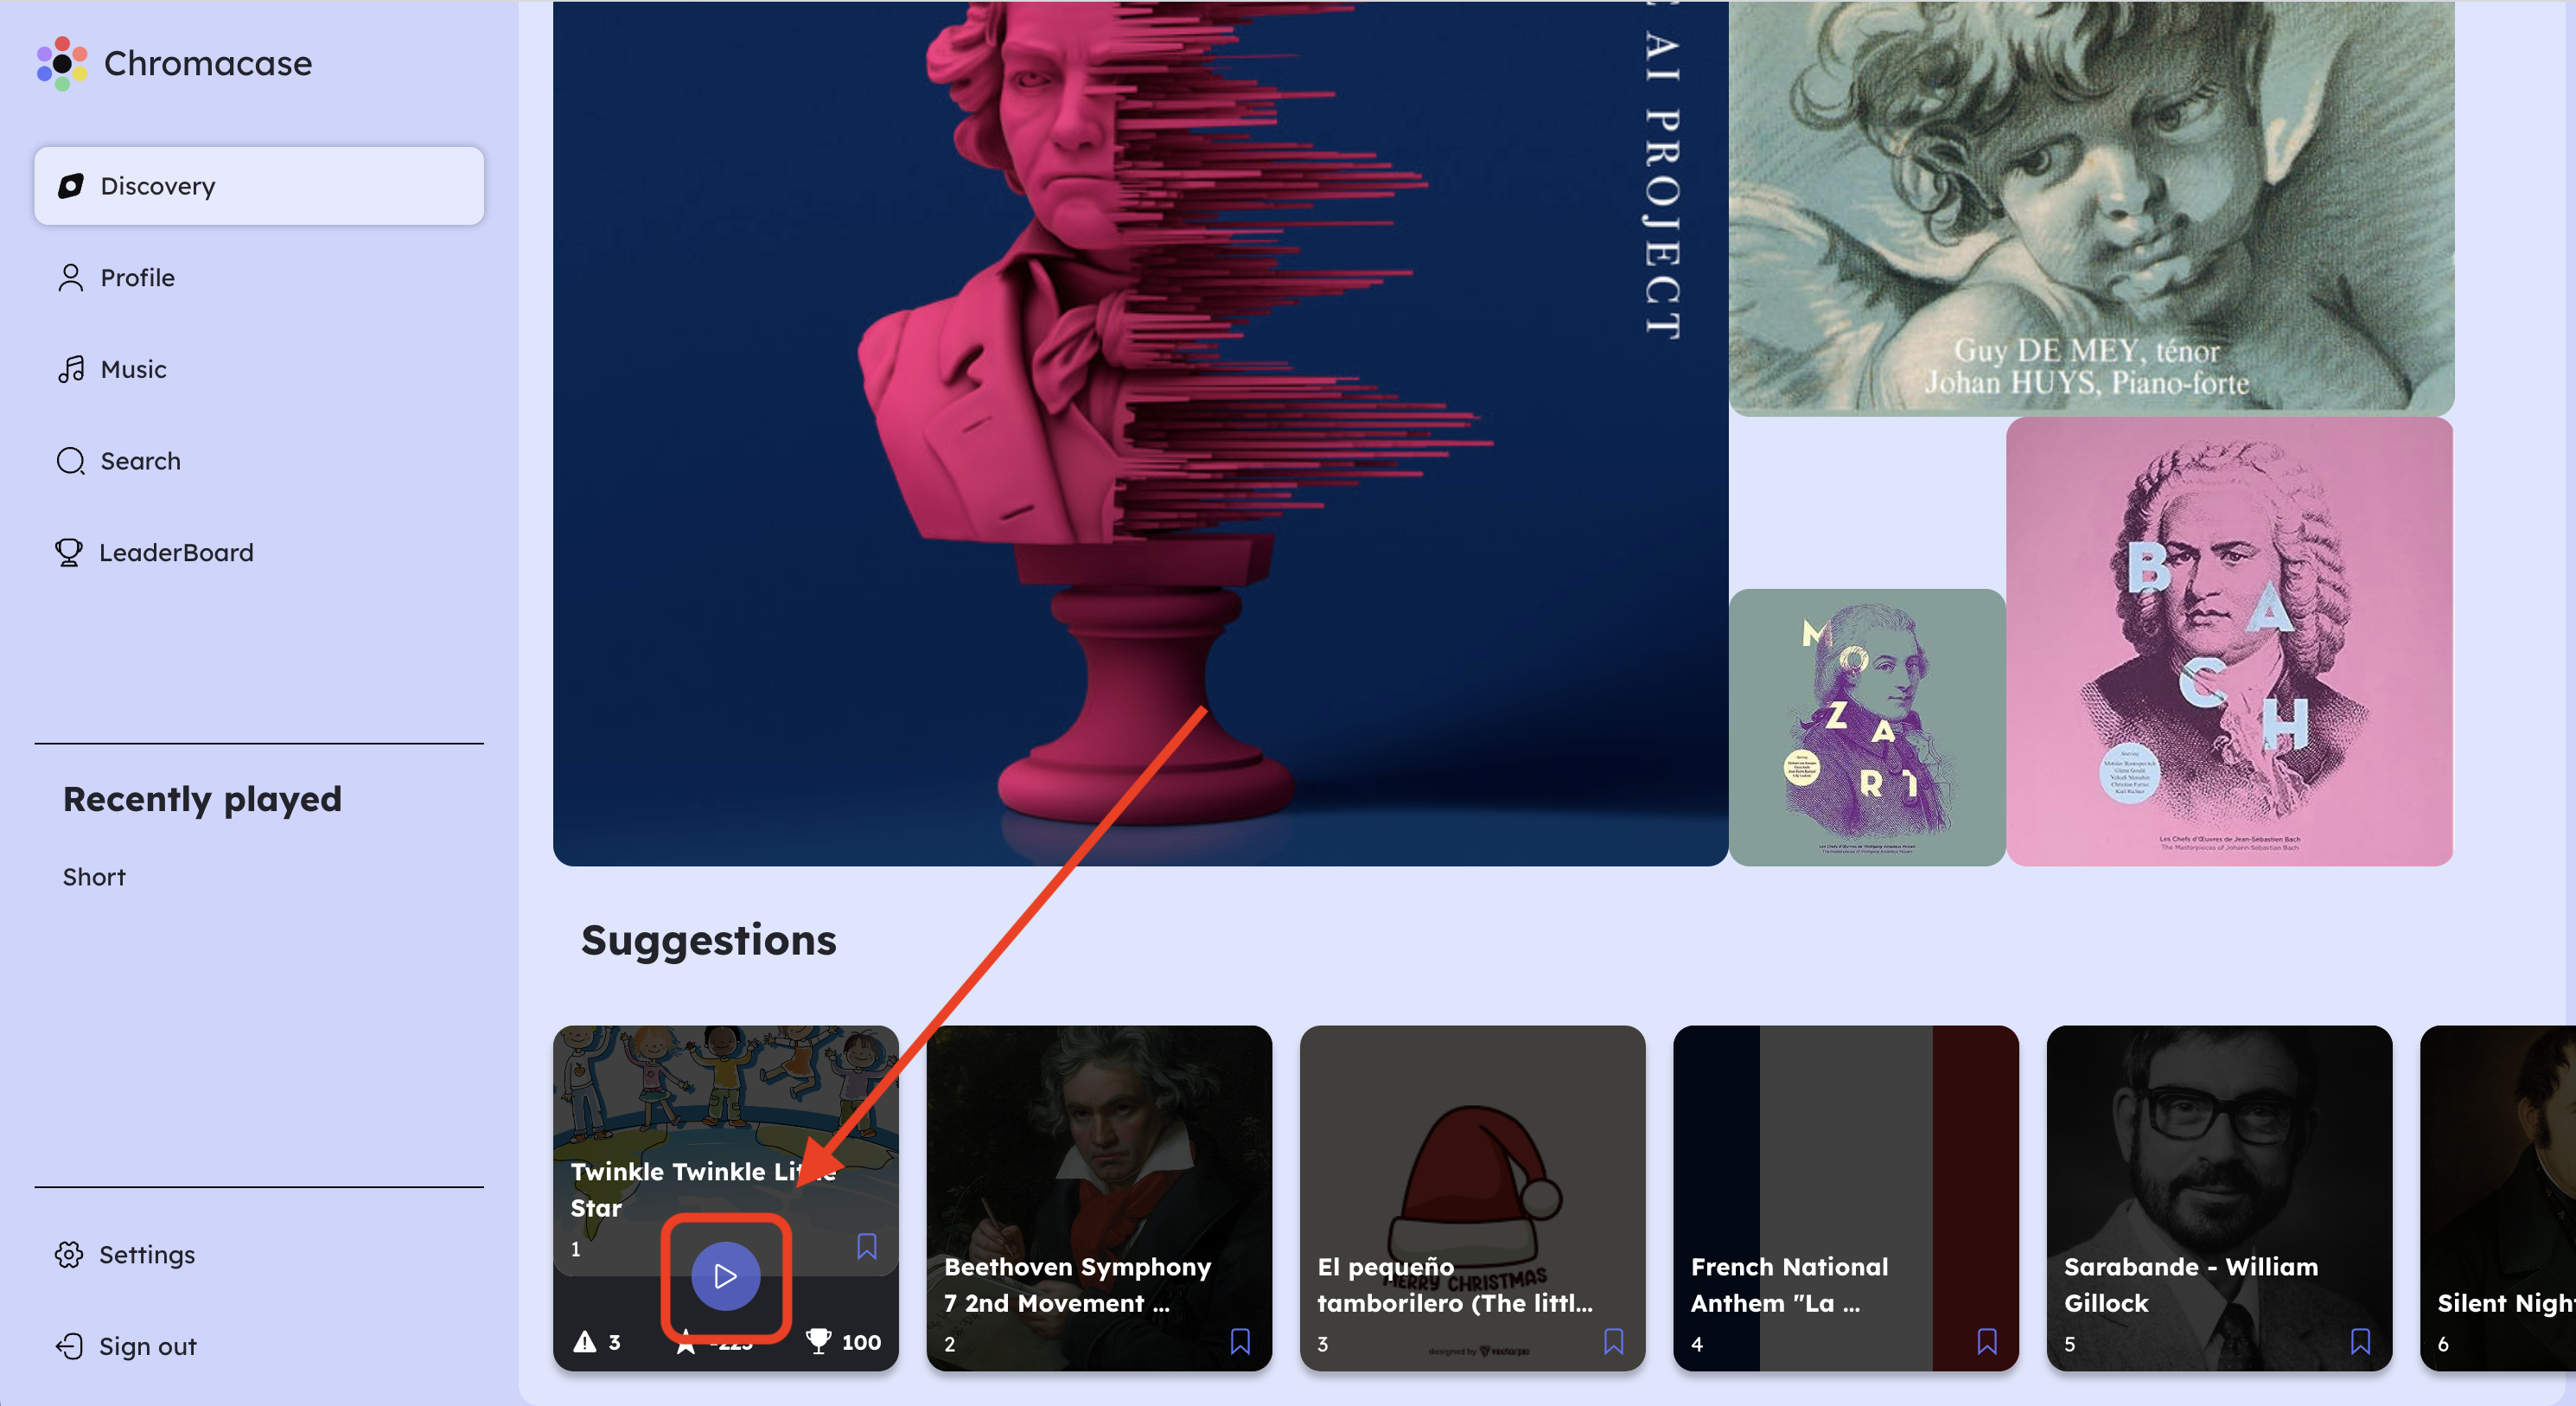
\includegraphics[width=\linewidth]{../\dir/guide/play/home.png}
	\caption{Acceder à une chanson depuis la page d'accueil}
	\label{fig:access-song}
\end{figure}

\begin{figure}[H]
	\begin{subfigure}[b]{0.7\textwidth}
		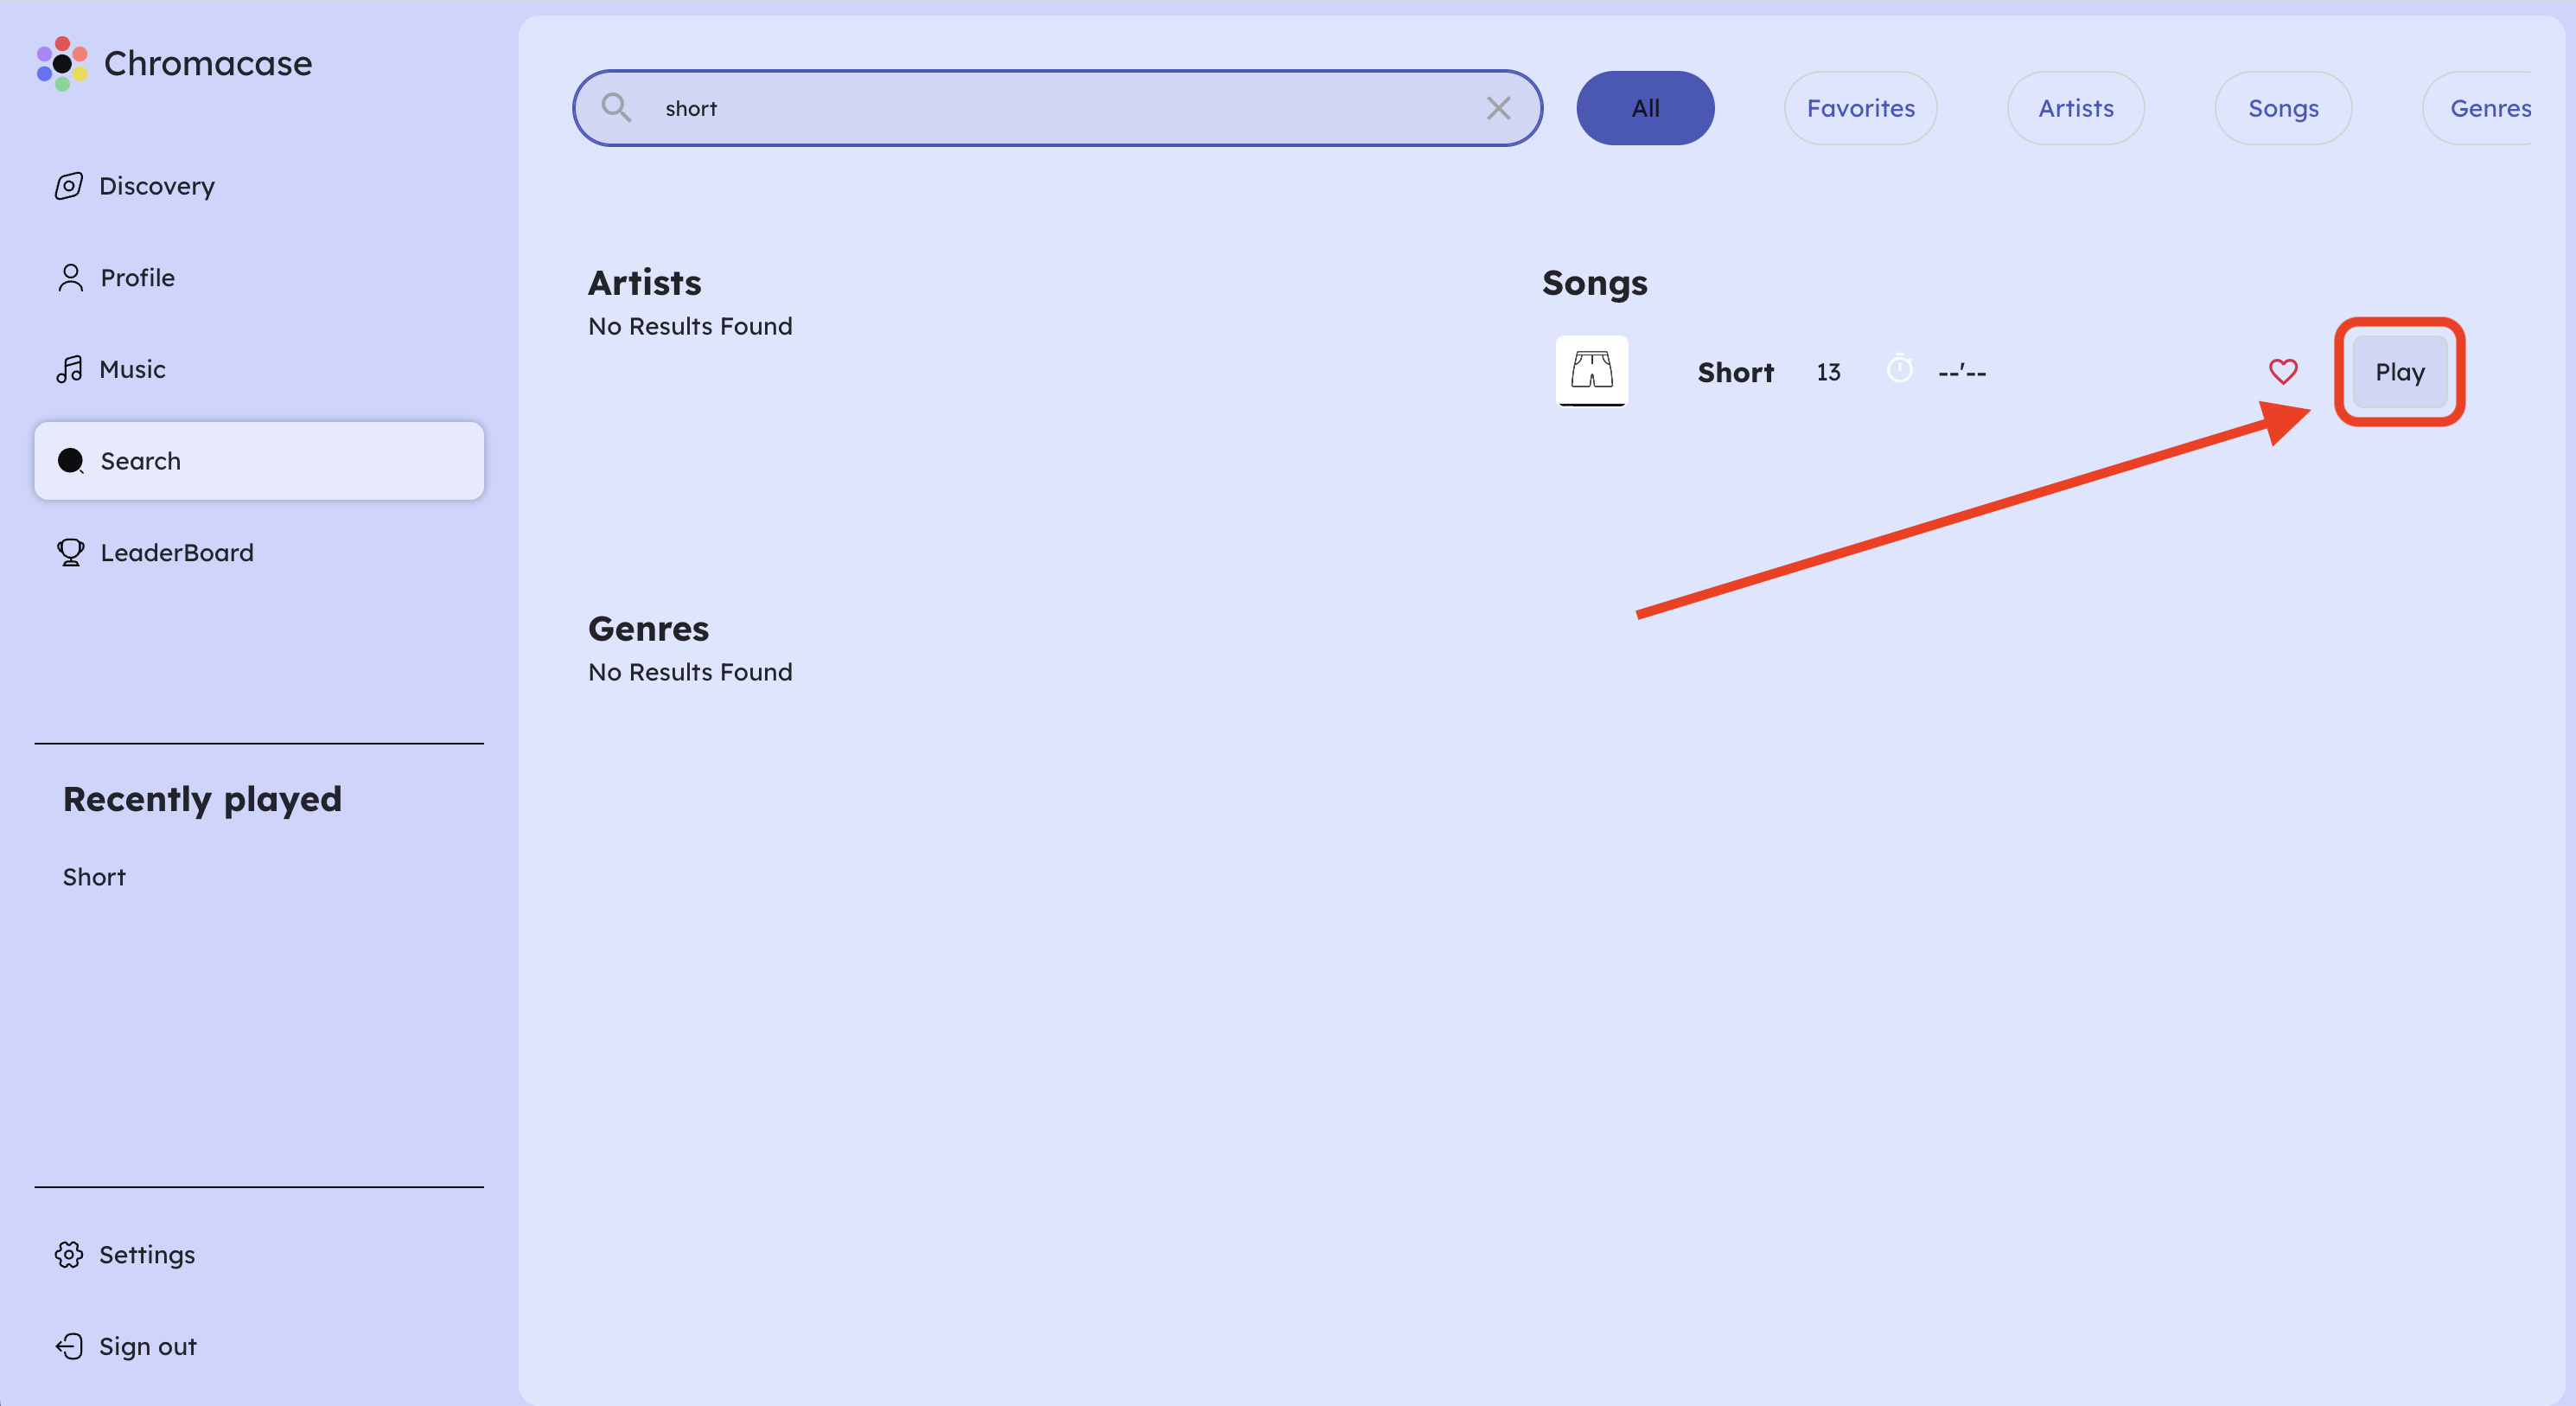
\includegraphics[width=\linewidth]{../\dir/guide/play/search.png}
		\caption{Version navigateur}
	\end{subfigure}
	\begin{subfigure}[b]{0.25\textwidth}
		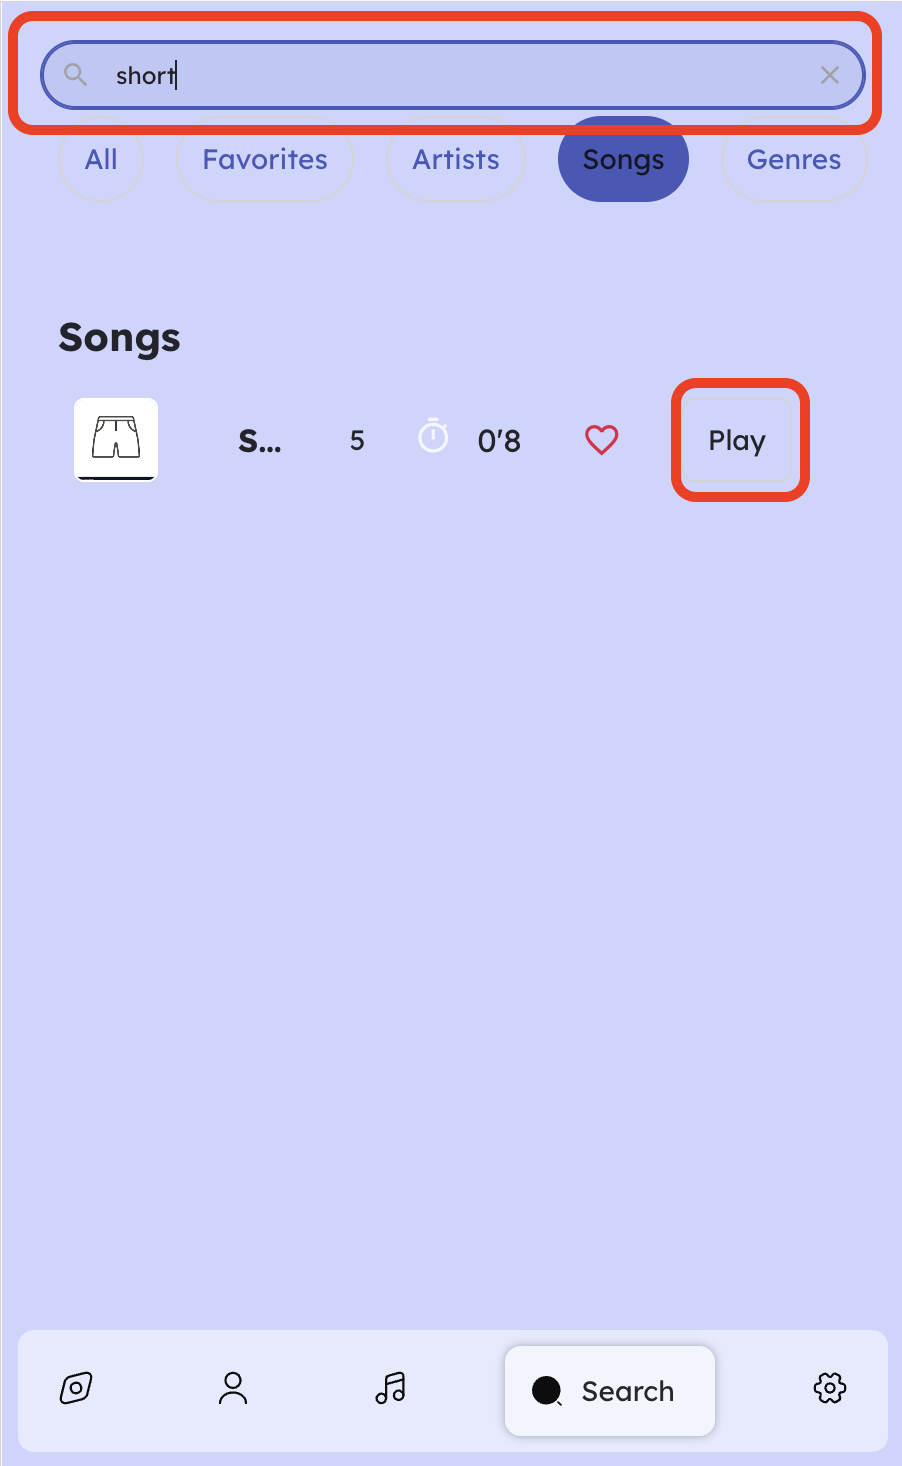
\includegraphics[width=\linewidth]{../\dir/guide/play/search-mobile.png}
		\caption{Version mobile}
	\end{subfigure}
	\caption{Acceder à une chanson depuis la page de recherche}
	\label{fig:search-song}
\end{figure}

Vous arriverez sur une page de lobby, où vous pouvez choisir le mode de jeu:

\begin{itemize}
	\item[Play] Mode de jeu normal: jouez toutes les notes au bon moment, au bon rythme.
	\item[Practice] Similaire au mode normal. Seul les notes sont importantes, pas le rythme.
\end{itemize}

Avant de lancer la partie, assurez-vous que votre piano MIDI soit connecté.
Cliquez sur l'un des boutons pour jouer (Voir Capture \ref{fig:choose-play-mode}).

\begin{figure}[H]
	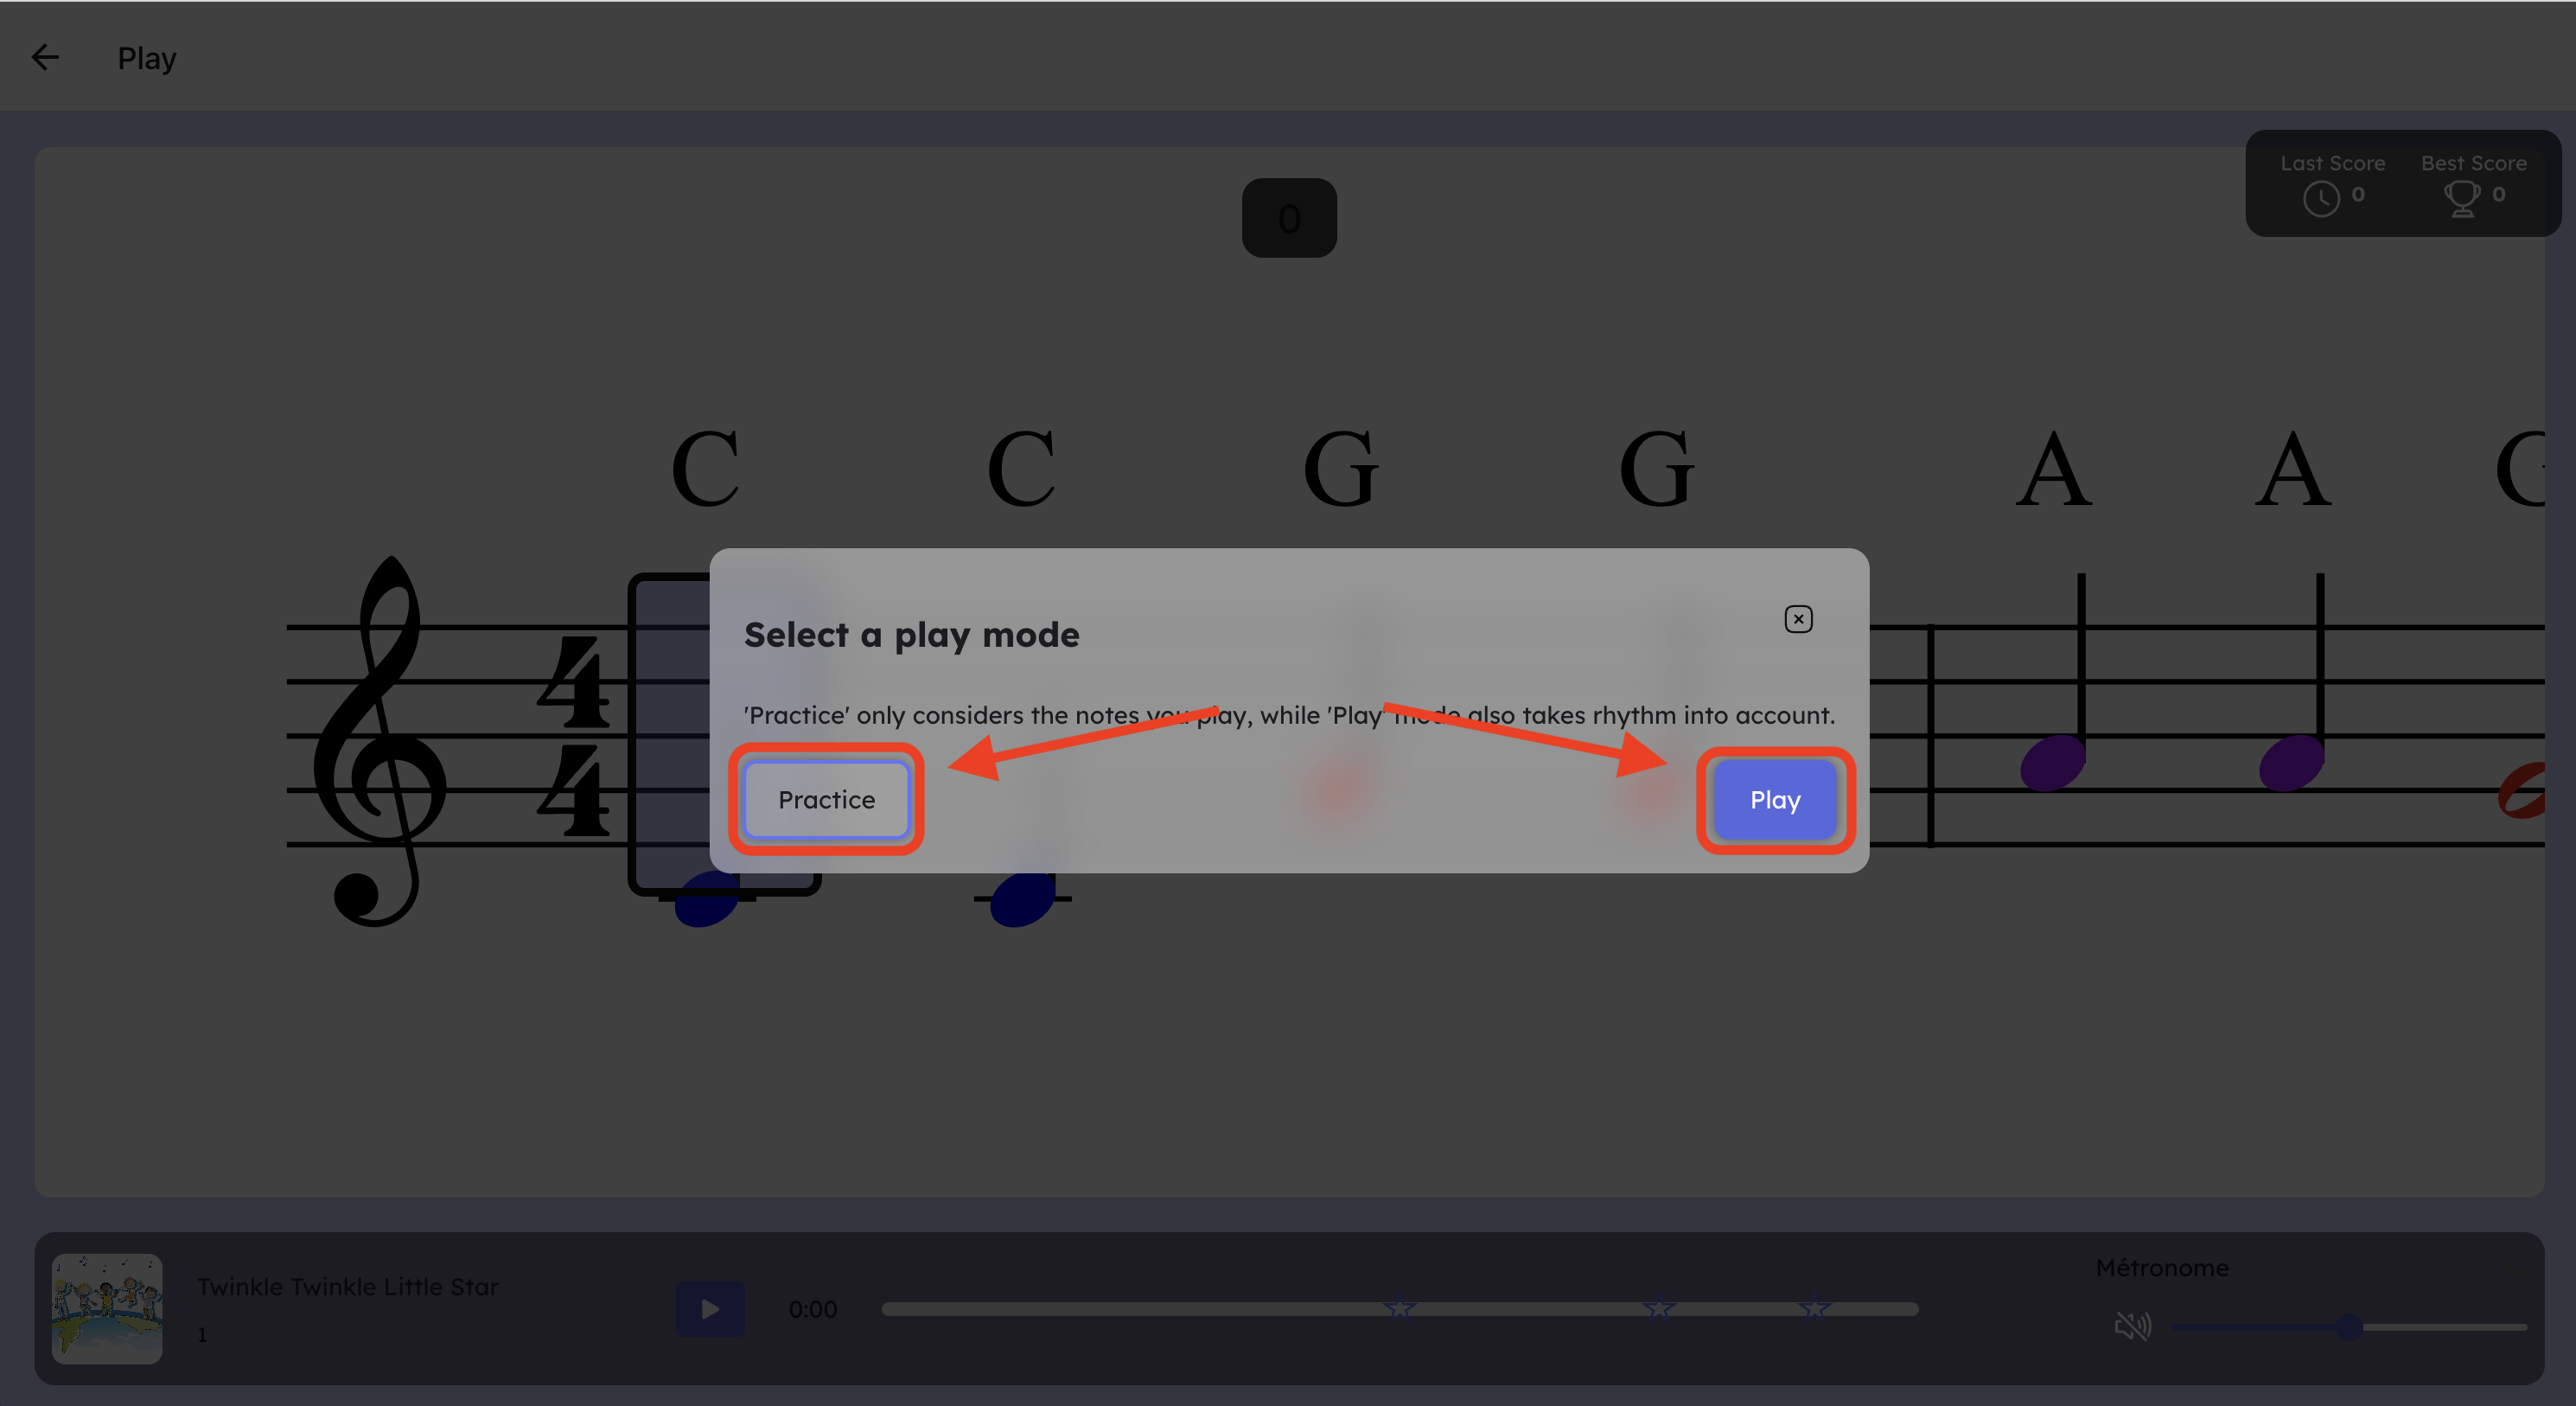
\includegraphics[width=\linewidth]{../\dir/guide/play/lobby.png}
	\caption{Lancer la partie depuis l'écran de lobby}
	\label{fig:choose-play-mode}
\end{figure}

Pour lancer la partie, cliquez sur le bouton Play. Un compte à rebours de 3 secondes sera lancé. Lorsque celui-ci sera écoulé, la partie commencera, et la partition défilera.

A tout moment, vous pouvez mettre la partie en pause avec le bouton Play/Pause dans la partie inferieure gauche de l'écran (Voir Capture \ref{fig:play}).

Le bouton "Metronome" en bas à droite vous permettent d'activer / désactiver le métronome, ainsi que de regler son volume (Voir Capture \ref{fig:play}).

Les notes sous le curseur sont les notes à jouer. Si vous jouez les notes correctement, le nombre de points gagnés augmentera.

\begin{figure}[H]
	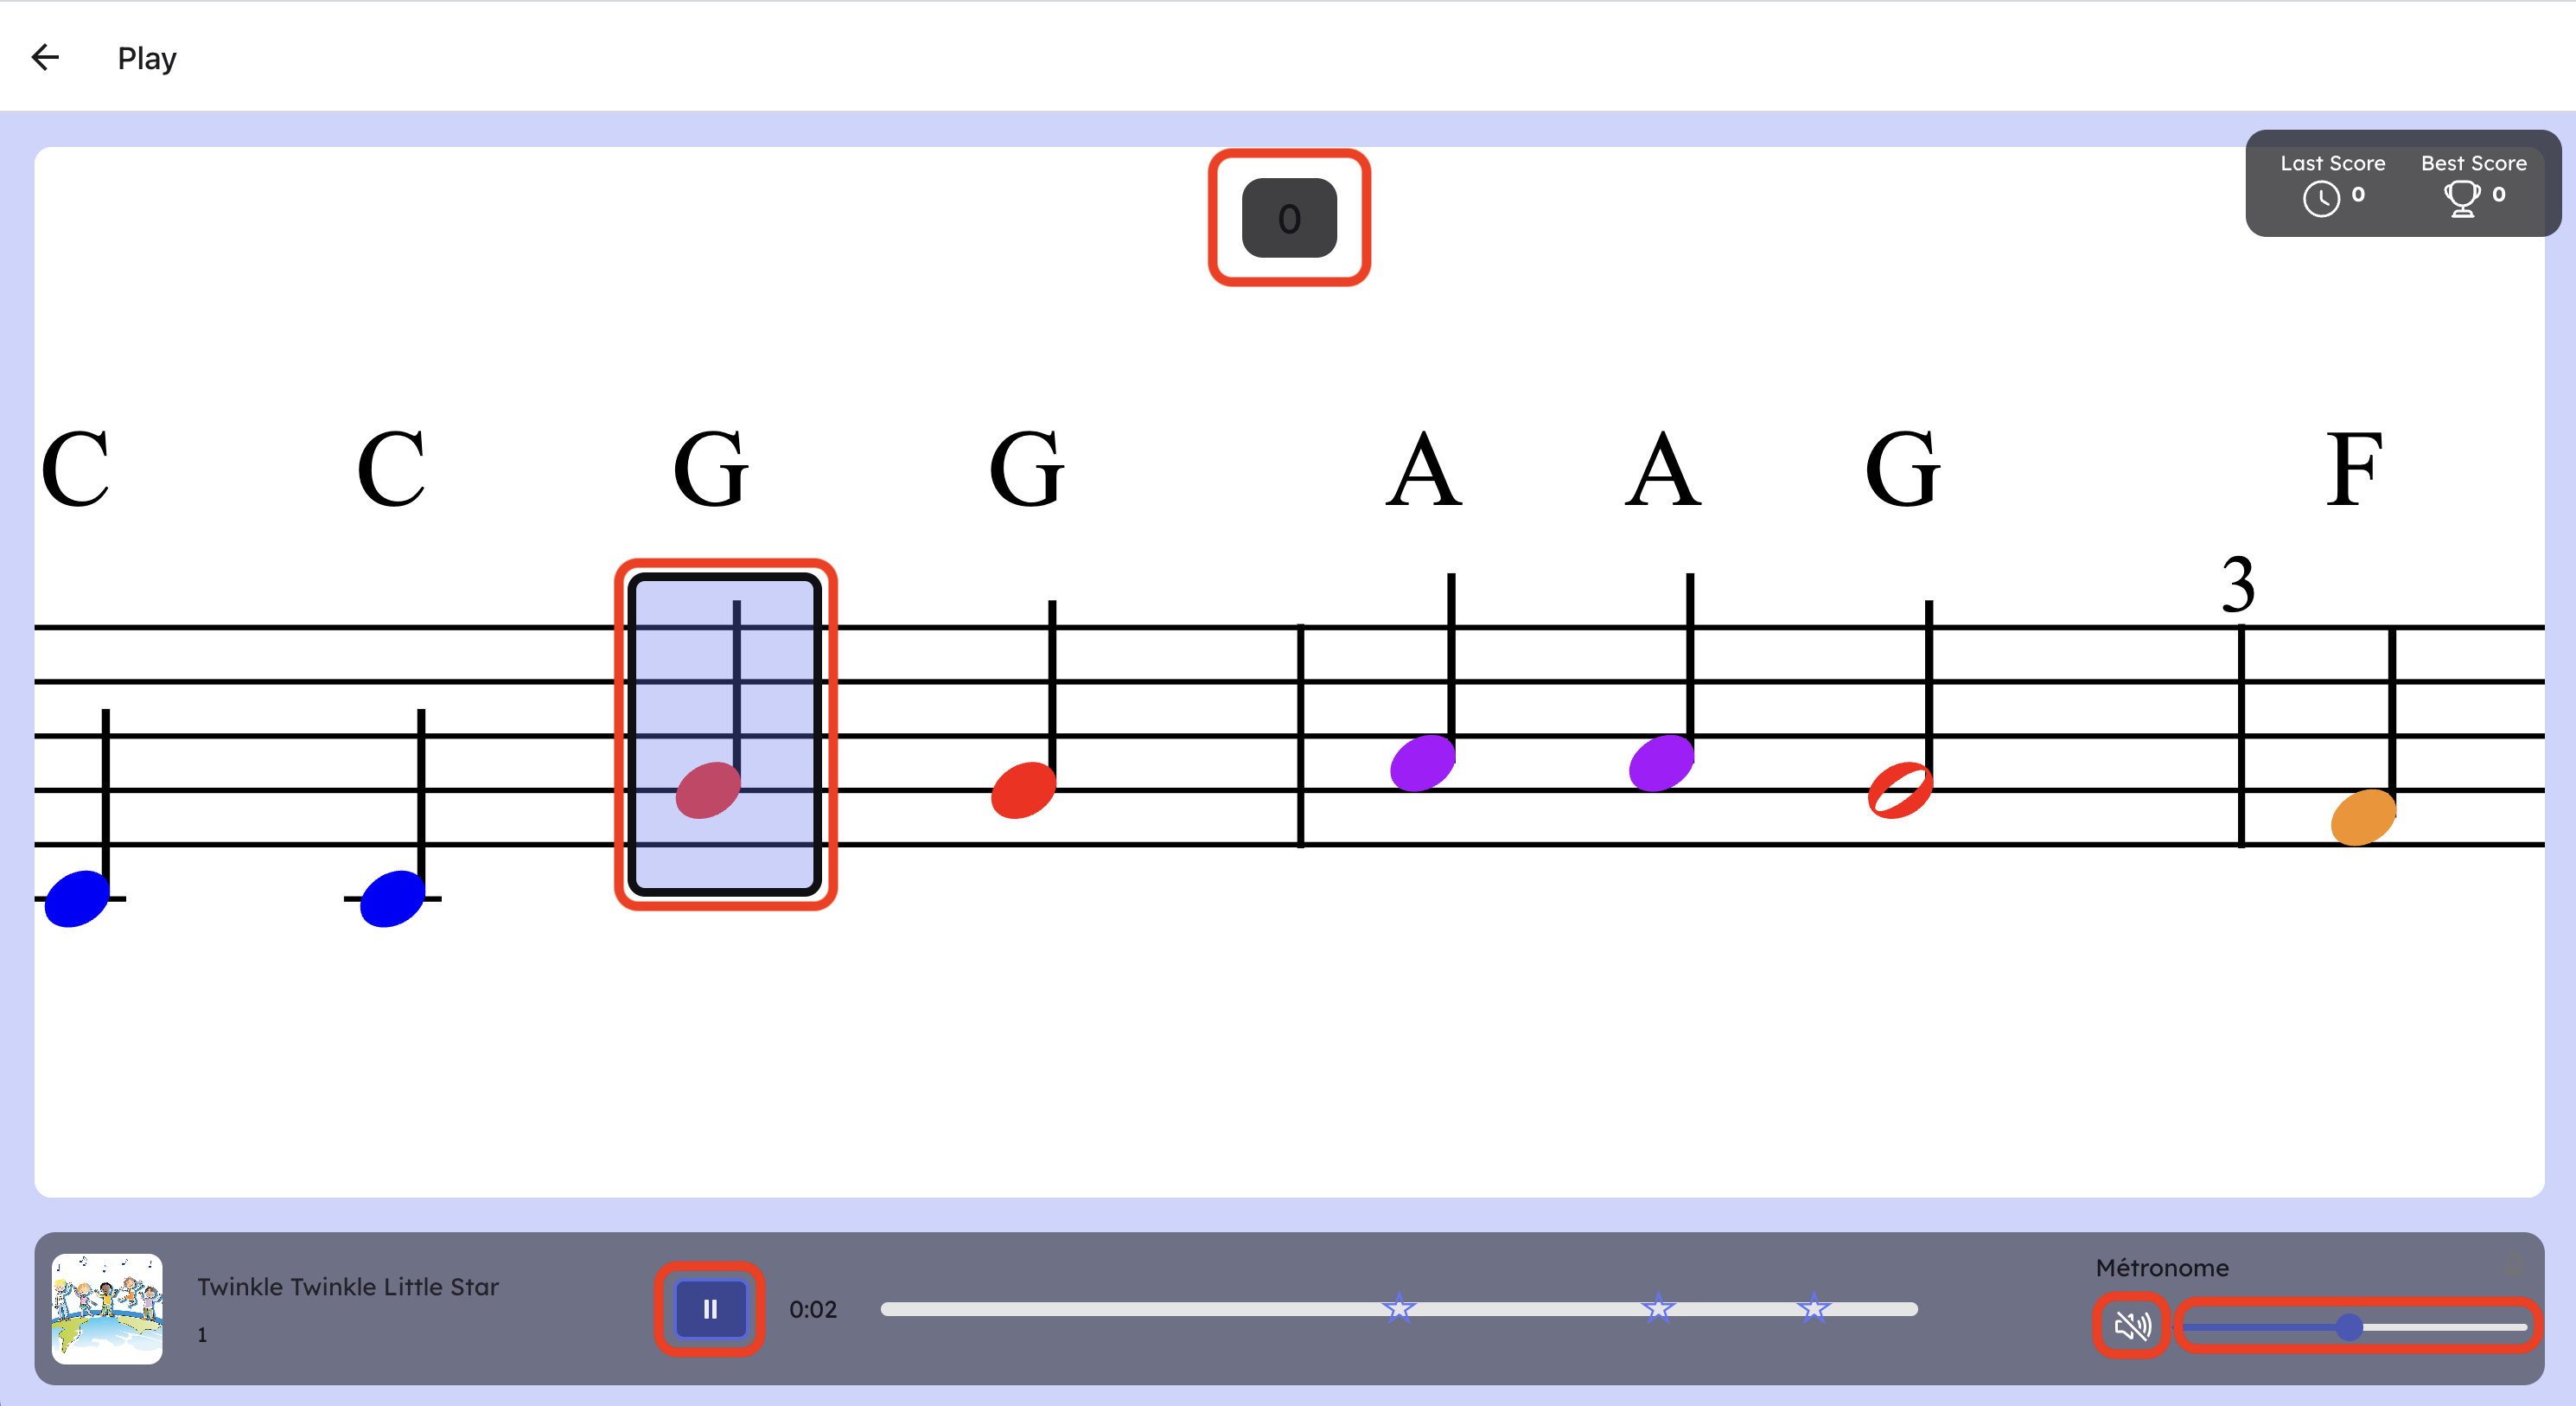
\includegraphics[width=\linewidth]{../\dir/guide/play/play.png}
	\caption{Lancer la partie}
	\label{fig:play}
\end{figure}

Vous pouvez faire pause à tout moment en cliquant sur le bouton pause. Vous pouvez stopper la partie en cliquant sur le bouton Stop.
\\\\
Une fois la partie terminée, vous pourrez avoir un apercu de votre score (Voir Capture \ref{fig:score}).

\begin{figure}[H]
	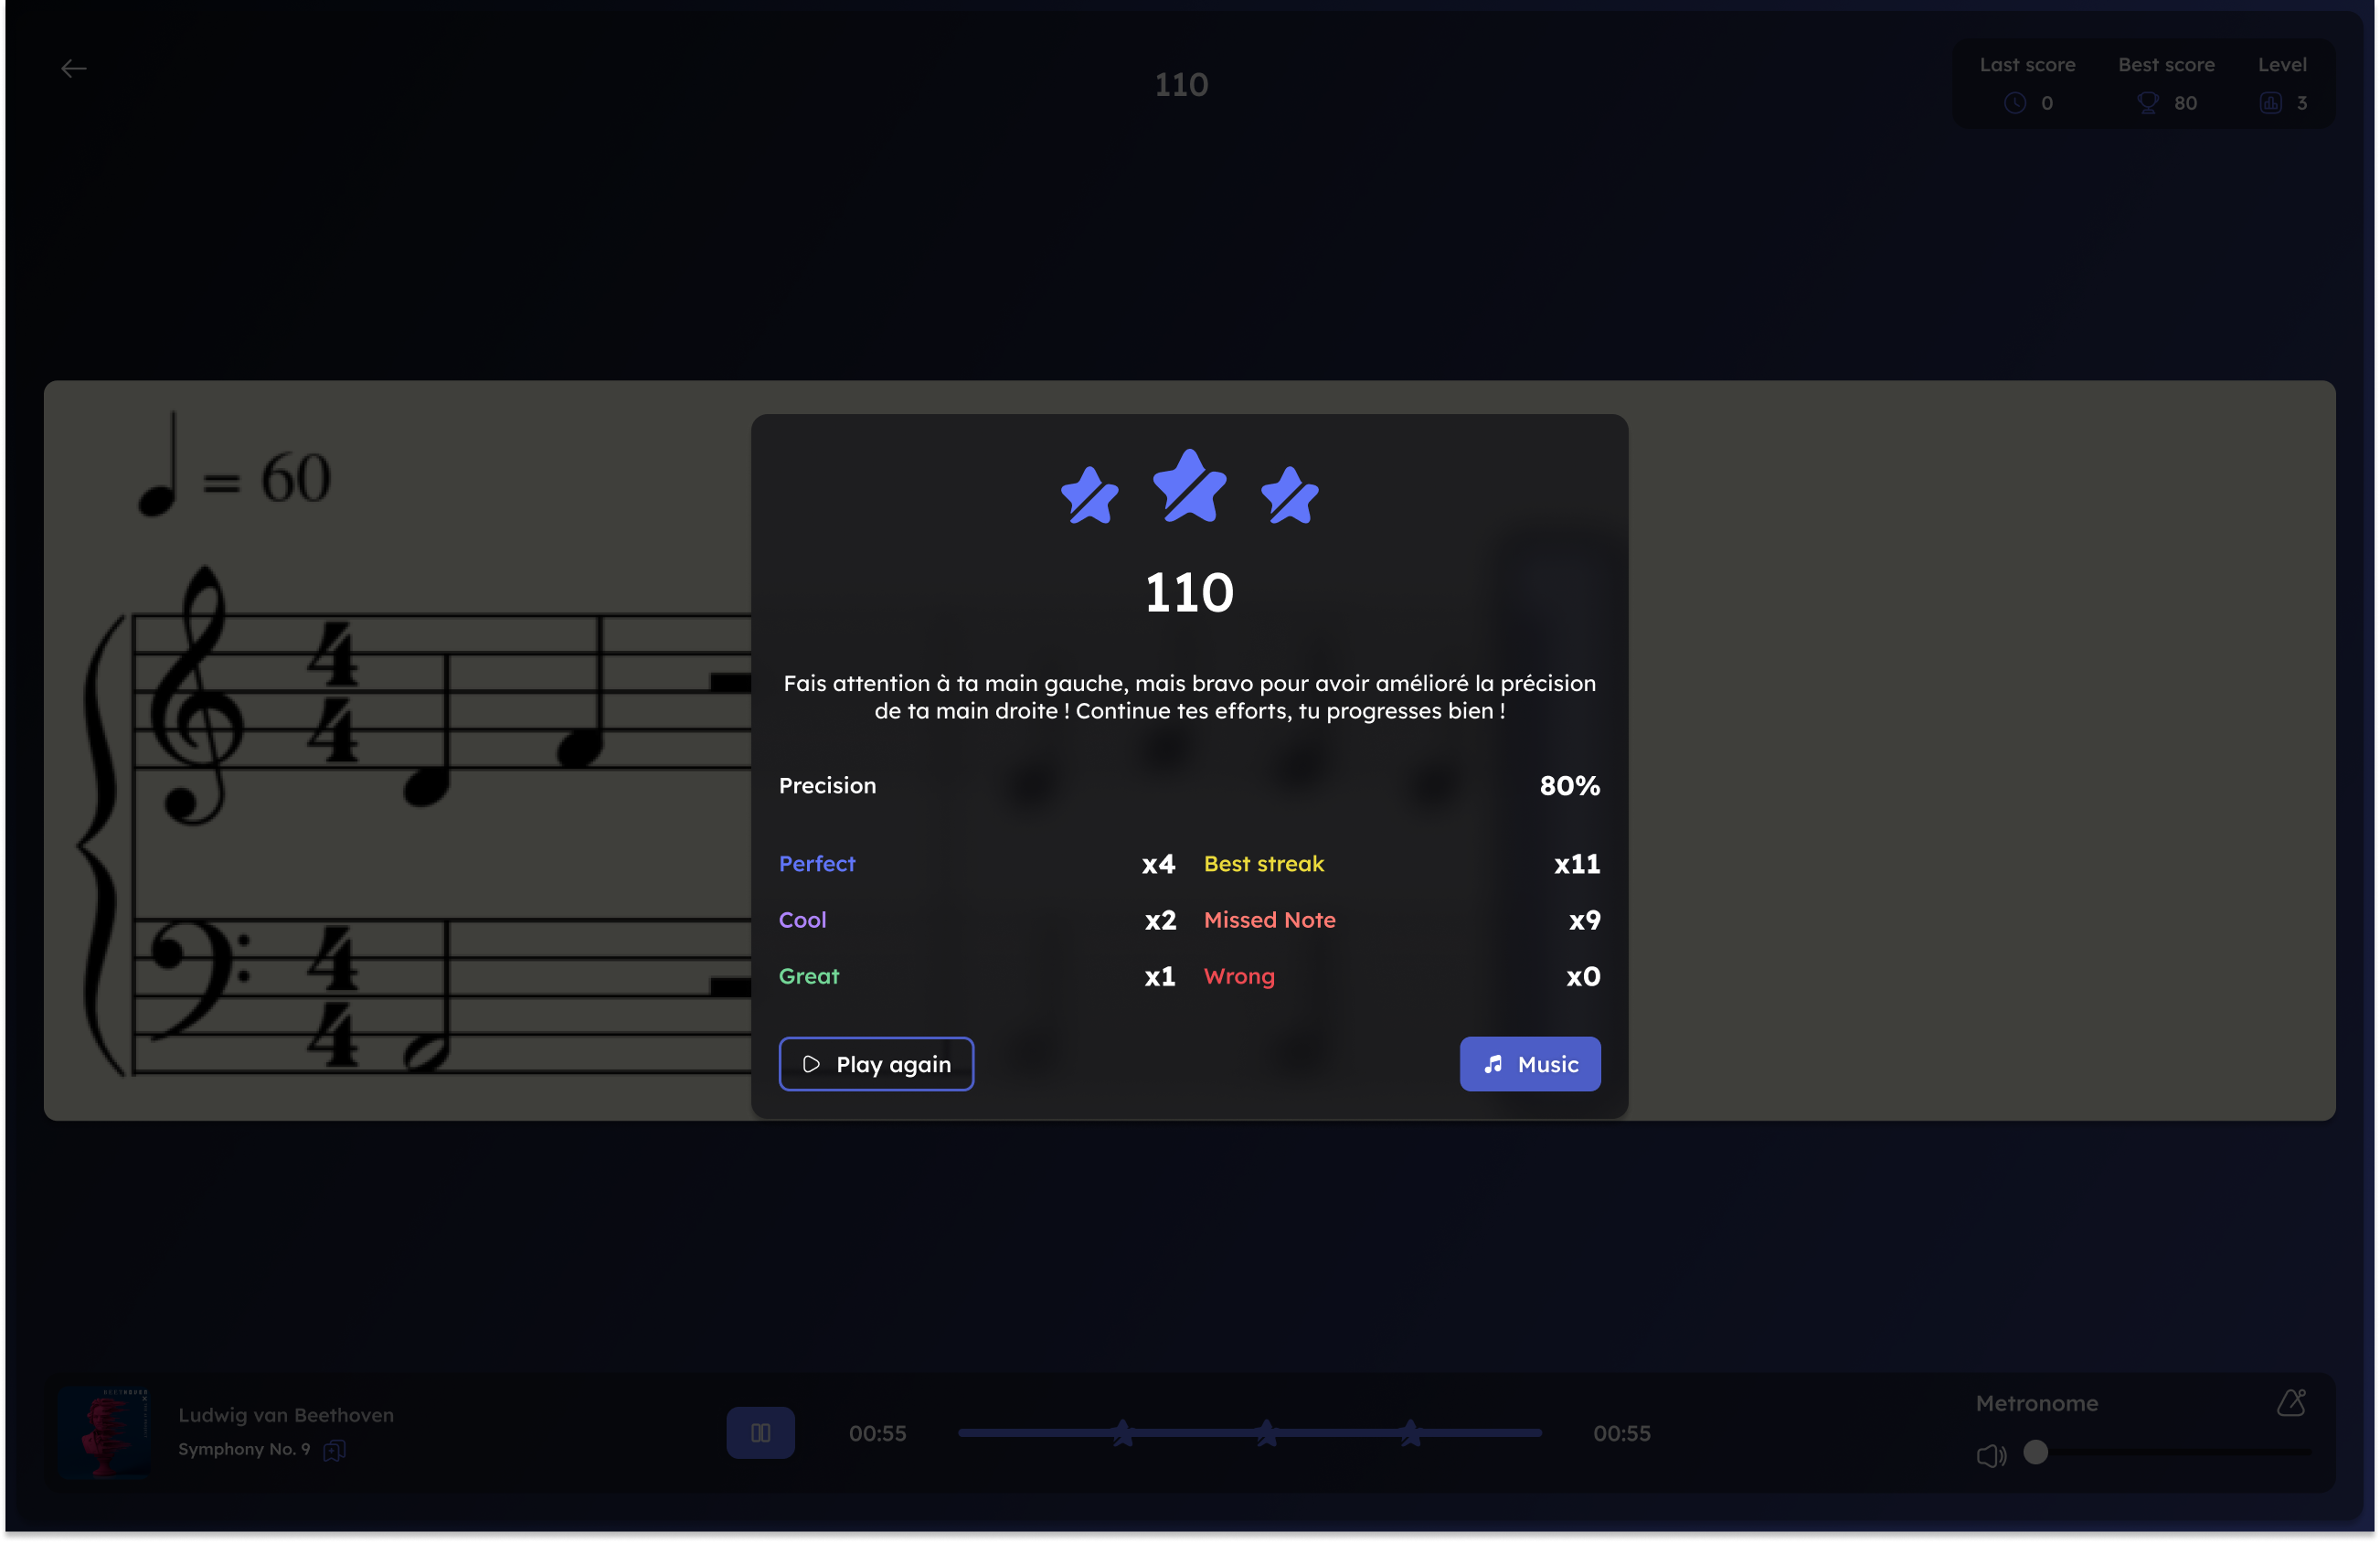
\includegraphics[width=\linewidth]{../\dir/guide/play/score.png}
	\caption{Score en fin de partie}
	\label{fig:score}
\end{figure}